\documentclass{beamer}
\usepackage[utf8]{inputenc}
\usepackage[T1]{fontenc}
\usepackage[french]{babel}
\usepackage{amsmath,amsfonts,amssymb}
\usepackage{graphicx}

\usetheme{Warsaw}

\author{Aurèle Barrière \& Nathan Thomasset}
\title{Cryptographie}
\date{10 mars 2016}


\begin{document}

\begin{frame}
\maketitle
\end{frame}

\begin{frame}{Mise en situation}
  \end{frame}

\begin{frame}{Intérêt de la cryptographie}
  Cartes bleues

  Mail

  Transaction bancaires
\end{frame}

\begin{frame}{Un codage ultime?}
  Seul quelqu'un qui connaitraît la clé pourrait décoder.
  \end{frame}

\begin{frame}{Exemple : chiffrement de César}
  Décalage.

  Exemple.
\end{frame}

\begin{frame}{Veni Vidi Decrypti}
  26 décalages possibles.
  \end{frame}

\begin{frame}{Énumération des clés}
  Énumérer les clés possibles (décalages). Regarder tous les résultats.
  \end{frame}

\begin{frame}{Complexité}
  Le calcul, c'est pas gratuit.

  Trop de clés -> trop de calcul, trop de résultats
  
  \begin{figure}
  \centering
  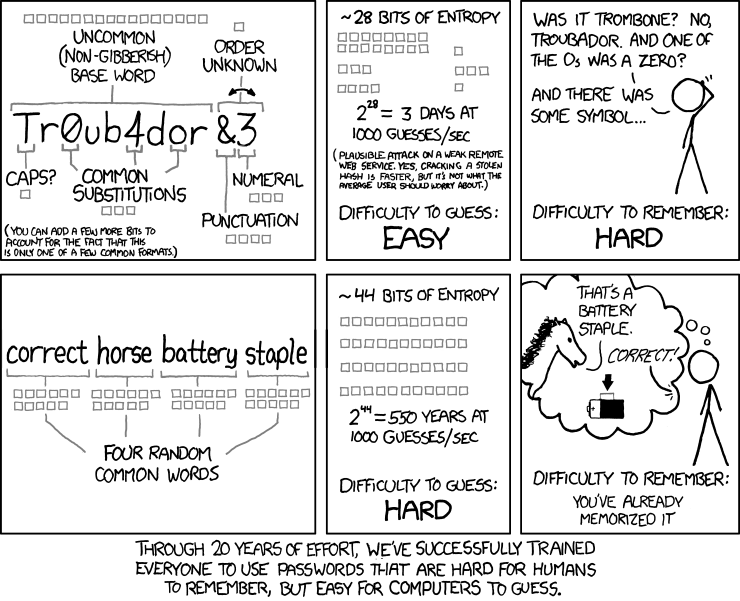
\includegraphics[scale = 0.35]{xkcdpassword_strength.png}
  \end{figure}
  \end{frame}

\begin{frame}{D'autres exemples}
  Hill

  Vigenere
  \end{frame}

\begin{frame}{Analyse fréquentielle}
  Chiffres pour matrices de Hill

  Fréquences français
  \end{frame}


\begin{frame}{Cryptographie asymétrique}
  Clé publique, clé privée

  Mise en situation
\end{frame}

\begin{frame}{RSA}
  Schéma
  \end{frame}

\begin{frame}{Limites}
  \begin{figure}
    \centering
    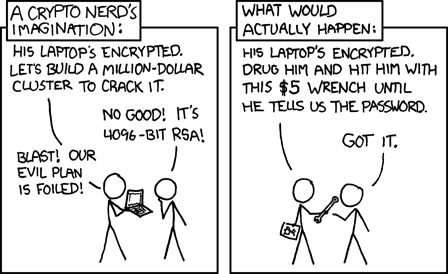
\includegraphics[scale = 0.5]{xkcdsecurity.png}
  \end{figure}
\end{frame}

\begin{frame}{Ressources et idées}
  GPG mail
  
  sources des images
  \end{frame}





\end{document}
